%----------------------------------------------------------------------------------------
%	ANALISI ARCHITETTURALE
%----------------------------------------------------------------------------------------

\section{Analisi architetturale}
\label{sec:analisi_architetturale}

In questo capitolo verranno presentate le decisioni architetturali inerenti la struttura e l'organizzazione del software di simulazione. L'analisi comincia con una visione generale della gerarchia di eventi, per poi suddividersi nelle scelte che riguardano la parte di concorrenza e le scelte che riguardano la parte di distribuzione.

\subsection{Gli eventi}
\label{sec:analisi_eventi}

Gli eventi sono l'elemento costituente di una partita. Essi vengono generati dalle diverse entità e possono essere raggruppati in diverse categorie. Inoltre, alcuni di questi eventi interessano la sola parte concorrente, mentre altri eventi possono viaggiare dalla parte concorrente a quella distribuita e viceversa.

\begin{figure}[htp!]
	\centering
	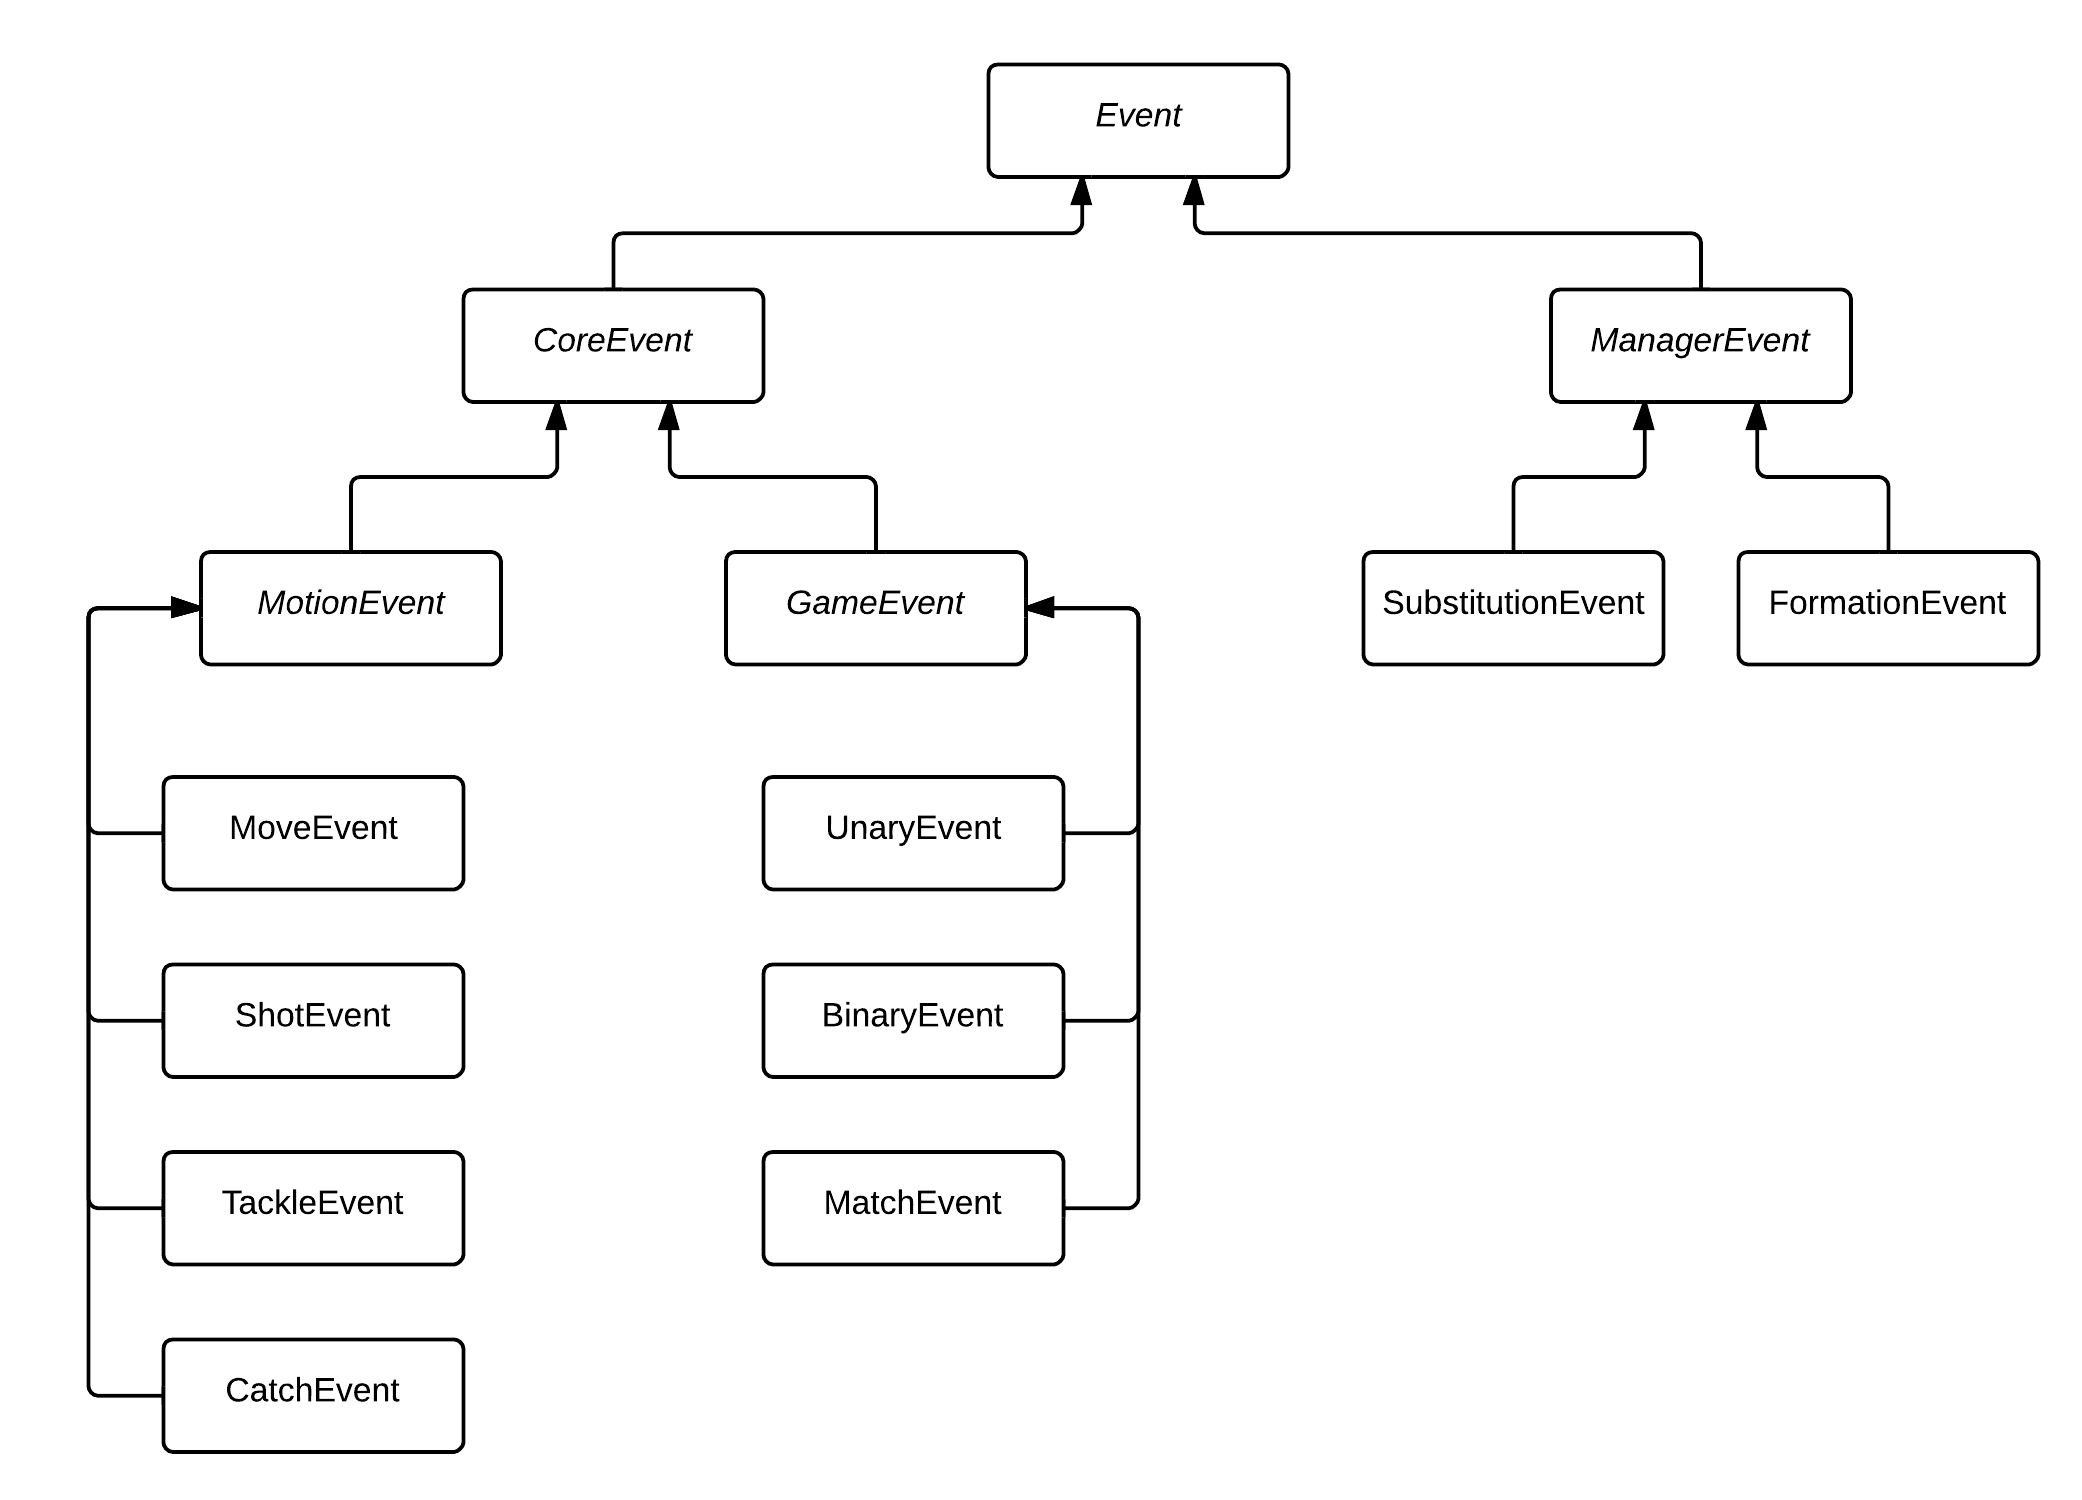
\includegraphics[scale=.2]{images/event_hierarchy.png}
	\caption{La gerarchia degli eventi che costituiscono una partita.}
	\label{fig:event_hierarchy}
\end{figure}

La struttura globale degli eventi è schematizzata in Figura~\ref{fig:event_hierarchy}. Data la sua complessità ed estensione, verranno ora trattati singolarmente i diversi tipi di eventi al fine di spiegarne il loro significato e il contesto in cui vengono utilizzati.

\paragraph{Event} \textit{Event} rappresenta l'evento generico ed è alla base della gerarchia. Da esso si diramano due macro-categorie di eventi: i \textit{CoreEvent} e i \textit{ManagerEvent}. Esso sono rispettivamente gli eventi che vengono generati nella parte concorrente (il \emph{Core}) e gli eventi che vengono generati nella parte distribuita (fondamentalmente, dagli allenatori). \textit{Event} può essere considerata come un'entità astratta, che non viene concretizzata se non da uno dei suoi derivati.

\paragraph{CoreEvent} Gli eventi di tipo \textit{CoreEvent} sono un insieme di eventi che vengono generati dalla parte concorrente del sistema. La loro generazione tuttavia non vincola il loro utilizzo nella sola parte concorrente: essi vengono infatti inviati alla parte distribuita per notificare gli allenatori (e l'interfaccia grafica del campo) aggiornamenti sullo svolgersi della partita. Vi sono due tipologie di \textit{CoreEvent}: i \textit{MotionEvent}, che rappresentano le possibili azioni dei giocatori, e i \textit{GameEvent}, che invece rappresentano tutti quegli eventi che influiscono sullo stato di gioco. Anche in questo caso, i \textit{CoreEvent} sono astratti e trovano una concretizzazione nei loro discendenti.

\paragraph{MotionEvent} Tutte le azioni che un giocatore può compiere sono definite dai \textit{MotionEvent}. Sono stati definiti quattro tipi di \textit{MotionEvent}, elencati di seguito.

\begin{itemize}
	\item \textit{MoveEvent} - descrivono i movimenti di un giocatore, dal punto in cui si trova al punto in cui si vuole spostare. Questi eventi vengono altresì usati per descrivere gli spostamenti della palla;
	\item \textit{ShotEvent} - rappresentano il tiro/passaggio effettuato da un giocatore, e sono caratterizzati da alcune informazioni quali la posizione del giocatore e la potenza impressa alla palla;
	\item \textit{TackleEvent} - corrisponde al tentativo di contrasto verso un altro giocatore;
	\item \textit{CatchEvent} - questo evento descrive il gesto di prendere possesso di una palla, sia essa inerte sul campo (non in possesso) oppure come intercettazione di una palla in movimento.
\end{itemize}

Ciascuno di questi eventi viene sottoposto all'attenzione dell'arbitro, che ne valida la correttezza nel rispetto delle regole del gioco. Inoltre, come già anticipato, questi eventi vengono anche inviati alla parte distribuita, così da poter aggiornare la visualizzazione della partita e per permettere agli allenatori di prendere decisioni tattiche.

\paragraph{GameEvent} Gli eventi che regolano lo svolgimento del gioco rientrano nella categoria di \textit{GameEvent}. Essendo una tipologia di evento molto vasta, esso si suddivide ulteriormente in tre specializzazioni: gli \textit{UnaryEvent}, i \textit{BinaryEvent} ed i \textit{MatchEvent}. Le prime due tipologie si riferiscono al fatto che l'evento coinvolge solamente un giocatore (e.g., una rimessa laterale: da qui, unario) oppure due giocatori (e.g. un fallo), mentre la terza tipologia raccoglie tutti gli eventi come l'inizio della partita, la fine del primo tempo, e così via.\\

\paragraph{UnaryEvent} Tutti gli eventi di gioco che sono raggruppati in questa categoria vanno a coinvolgere un solo giocatore per la ripresa del gioco. Essi rappresentano le seguenti situazioni:

\begin{itemize}
	\item rimessa laterale;
	\item rimessa dal fondo;
	\item calcio d'angolo;
	\item calcio di punizione;
	\item calcio di rigore.
\end{itemize}

Ciascuno di questi eventi prevede che il gioco possa essere sbloccato da un particolare giocatore della squadra interessata e che la palla sia posizionata nella posizione stabilita dall'arbitro. Il gioco può riprendere solo se i giocatori sono nella loro posizione di riferimento per quella particolare situazione, prima che la palla venga rimessa in gioco. Inoltre, questi eventi sono generati esclusivamente dall'arbitro, che per ogni azione effettuata controlla lo stato di gioco globale alla ricerca di irregolarità.

\paragraph{BinaryEvent} Questa particolare categoria vanta un solo evento possibile: il fallo. Questo evento è infatti l'unico a coinvolgere simultaneamente due giocatori di squadre opposte, e si origina quando il contrasto avviene in maniera irregolare (infortuna il giocatore, oppure compie gesti pericolosi). In questo caso l'arbitro, dopo aver segnalato del fallo, decide le modalità di ripresa del gioco, ad esempio un calcio di punizione, e genera il rispettivo evento.

\paragraph{MatchEvent} Gli eventi che regolano l'inizio e la fine di ciascun tempo di gioco fanno parte dei \textit{MatchEvent}. Di conseguenza, vi sono quattro possibili varianti: inizio del primo tempo, fine del primo tempo, inizio del secondo tempo, fine del secondo tempo. Questi eventi sono usati sia dai giocatori per capire quale azione dovranno compiere (e.g., ingresso in campo), ma vengono anche inviati alle componenti distribuite per notificare lo svolgersi della partita.

\paragraph{ManagerEvent} Questa classe astratta di eventi, al contrario dei \textit{CoreEvent} che sono generati dalla componente \textit{Core}, vengono generati dalle componenti distribuite, in particolar modo dai due \textit{Manager}. La loro funzione è quella di notificare all'arbitro una richiesta di sostituzione per un giocatore oppure di cambio di formazione. L'arbitro, una volta ricevuto l'evento, provvederà ad elaborarlo alla prima occasione utile di gioco fermo.\\

Un \textit{SubstitutionEvent} contiene informazioni quali la squadra interessata, il numero di maglia del giocatore uscente e il numero di maglia del giocatore entrante; un \textit{FormationEvent} invece, oltre alla squadra interessata, fornisce anche una sigla identificativa del nuovo assetto che la squadra dovrà assumere.

\subsection{Concorrenza}
\label{sec:analisi_concorrenza}

Questa sezione propone inizialmente una panoramica sulla soluzione scelta per garantire l'assenza di deadlock e starvation in fase di design. Successivamente viene fatta luce su casi particolari che il modello finora descritto non gestisce, mettendo in evidenza la necessità di arricchirlo con meccanismi e componenti dedicate.\\

La scelta del linguaggio per lo sviluppo della parte principale del software è ricaduta su Ada, il quale ha un modello di concorrenza che mette a disposizione una semantica molto ricca. Un aspetto molto interessante riguarda i canali di comunicazione per le richieste: questi permettono accessi potenzialmente paralleli in fase di lettura, mentre  garantiscono mutua esclusione e, in alcuni casi, anche accodamento condizionale in scrittura. Quest'ultimo costrutto è molto utile quando si vuole soddisfare una richiesta solamente al verificarsi di alcune condizioni, come per esempio una risorsa che si libera o una variazione dello stato di gioco.

\subsubsection{Deadlock, starvation e correttezza}
\label{sec:analisi_concorrenza_deadlock}

In un sistema concorrente è necessario tenere conto di problematiche come la starvation ed il deadlock, specialmente quando si è in presenza di entità che condividono risorse. Nel caso di questo progetto, i giocatori devono avere accesso ad uno stato condiviso che gli permetta di prendere decisioni, le quali andranno poi a modificare lo stato stesso.\\

L'analisi del problema ha evidenziato la necessità di avere un unico luogo in cui mantenere lo stato. In fase di modellazione, tale problematica è stata risolta ponendo un'unica entità che garantisce mutua esclusione al controllore dei dati condivisi.\\

Questa decisione rende più semplice garantire l'assenza di deadlock e di starvation. Nel secondo caso, ogni job ha la garanzia di accedere alla risorsa in un tempo finito, in quanto le richieste vengono processate con ordinamento FIFO basato sul tempo di arrivo. Per quanto riguarda invece il primo caso, è presente solamente uno dei quattro requisiti che stanno alla base di questa pericolosa condizione. I giocatori eseguono la propria sequenza di operazioni (che caratterizza un turno) dividendole tra ``online'' ed ``offline'': questo vuol dire che solamente le fasi di lettura e di scrittura necessitano dell'utilizzo della risorsa, mentre la parte di intelligenza artificiale viene effettuata in modo autonomo sui dati recuperati; inoltre, solamente la parte di scrittura richiede mutua esclusione. Il pre-rilascio non è inibito ed il suo comportamento non è controllato dal software, ma dal sistema operativo operativo sottostante: un job pre-rilasciato che sta eseguendo la sezione critica di una richiesta in mutua esclusione deterrà ancora, al suo risveglio, il privilegio sulla risorsa, mentre gli altri job che la richiedono saranno in attesa sul rispettivo canale esposto.\\

Un caso più particolare si ha invece per quanto riguarda attesa circolare ed accumulo di risorse, per cui entra in gioco un meccanismo di riaccodamento e rivalutazione delle richieste che verrà discusso in seguito. Per ora, basti sapere il concetto alla base di tale meccanismo: una richiesta che non viene soddisfatta a causa di una risorsa occupata può fallire o venire riaccodata, così da poter effettuare un nuovo tentativo di esecuzione in un secondo momento. In questo caso, dopo un certo numero di tentativi, l'operazione viene rivalutata e modificata in una simile, che vada comunque a soddisfare le esigenze del giocatore.

\subsubsection{Palla}
\label{sec:analisi_concorrenza_palla}

La palla consiste di una risorsa protetta che ne detiene la posizione e ne permette l'accesso in mutua esclusione. Si supponga di tenere tale risorsa all'interno del controllore, permettendo solo ad esso di accedervi: in questo caso, sia i giocatori che l'agente di movimento dovrebbero concorrere per andare a modificare lo stato e, di conseguenza, anche la posizione della palla: il moto della palla sarebbe quindi posto allo stesso livello delle decisioni e degli spostamenti dei giocatori. In queste circostanze verrebbe meno un fattore di realismo molto importante, tale per cui la palla è slegata dalla velocità di gioco dei giocatori in campo. Essa deve invece essere libera di muoversi a velocità molto più alte rispetto ai giocatori e deve poter continuare il proprio moto anche con gioco fermo: in quest'ultimo caso sarà l'arbitro a riposizionarla, ad esempio, in un punto opportuno a seconda dell'irregolarità. Inoltre, accodando una richiesta di movimento della palla insieme ad altre richieste dei giocatori, si rendono le operazioni strettamente sequenziali, eliminando un livello di indeterminismo desiderabile che è proprio del parallelismo e che lo avvicina al gioco reale.\\

Un chiaro esempio di questo aspetto si trova nel tentativo di un giocatore di prendere la palla in movimento. È ragionevole pensare che la sua azione possa fallire perché il tiro è troppo forte. Se invece si pongono la palla e lo stato in due luoghi differenti, diventa possibile uno scenario in cui il giocatore tenta di prendere la palla nell'ultima posizione a lui nota ma quest'ultima nel frattempo si è spostata.\\

Sulla base delle considerazioni fatte finora, all'interno dell'architettura è stato deciso di tenere le informazioni riguardanti la palla slegate rispetto al controllore. In questo modo si permette sia ad un giocatore che all'agente di movimento di contendere la palla in modo potenzialmente parallelo, demandando alla risorsa che identifica la palla gestirne gli accessi in mutua esclusione e sotto determinate circostanze.\\

La struttura della palla è stata quindi studiata in modo tale da permettere ad un entità alla volta di poterla controllare, sia essa uno dei giocatori (attraverso il controllore) oppure l'agente di movimento. Quest'ultimo si attiverà quando risvegliato da un giocatore e sarà fermato quando un altro giocatore conquista il pallone o se il moto che gli era stato impresso si è esaurito. In particolare, l'attivazione e disattivazione del task sfrutta la potenza dei canali che permettono accodamento con condizione.

\subsubsection{Giocatori}
\label{sec:analisi_concorrenza_giocatori}

I giocatori, dopo una prima fase di inizializzazione, eseguono ad ogni turno un'operazione che va a modificare sia lo stato di gioco che il proprio. Se ogni giocatore avesse la propria parte di stato, la sua condivisione con le altre entità in gioco sarebbe più complicata di quanto necessario; inoltre, la necessità di un unico stato centrale rende tali informazioni ridondanti oltre che difficilmente consistenti durante l'esecuzione della simulazione.\\

\textbf{Task stateless}\\

Utilizzando un approccio in cui i giocatori sono stateless si permette una migliore gestione dei dati condivisi, che vengono mantenuti in un unico luogo all'interno del sistema. Ad ognuno dei 22 task in campo viene assegnato un identificativo con il quale, ad ogni turno, il giocatore ottiene le informazioni che lo riguardano e di cui ha bisogno. Tale identificativo viene ottenuto in fase di inizializzazione e può cambiare solamente in caso di sostituzione tra un giocatore in campo ed uno in panchina; così facendo non vi è necessità di creare o risvegliare un secondo task.\\

\textbf{Area di azione}\\

Ogni giocatore è caratterizzato da alcune statistiche, impostate in fase di inizializzazione, che lo differenziano dagli altri: esse hanno come scopo quello di rendere lo svolgimento del gioco più realistico (Sezione~\ref{sec:analisi_giocatori}). Abbinate allo stato di gioco del giocatore stesso, rendono inoltre possibile effettuare alcune assunzioni che influiscono nello svolgimento del resto del turno.\\

Se un giocatore è in possesso della palla e tra le proprie statistiche ha un'alta precisione e potenza, esso potrà effettuare un lancio lungo e raggiungere compagni più distanti; in caso contrario, potrà sempre optare per un passaggio corto ad un compagno vicino. Viene definita in questo modo un'area di interesse del giocatore, entro la quale esso potrà agire a prescindere dall'azione che sceglierà di fare. Un giocatore che chiede al controllore lo stato di gioco della partita non necessita di avere una visione globale dell'intero campo, bensì solamente di una sua sotto parte, definita dalla sua posizione ed un raggio determinato in base alle caratteristiche del giocatore ed alle informazioni preliminari che ha ottenuto riguardo allo stato globale.\\

\textbf{Il turno}\\

La parte iniziale di ogni turno del giocatore risulta suddivisa come segue:

\begin{enumerate}
	\item richiesta al controllore del proprio stato di gioco;
	\item individuazione della posizione della palla;
	\item richiesta al controllore dello stato della propria area di interesse.
\end{enumerate}

Queste operazioni, in quanto letture, vengono effettuate potenzialmente in modo parallelo rispetto agli altri task.\\

La seconda fase consiste nella parte di intelligenza artificiale, nella quale viene decisa la prossima mossa da effettuare. Una volta decisa, viene creato il relativo evento a cui viene automaticamente abbinato un certo livello di utilità: questo valore determina quanto sia importante per il giocatore l'azione appena decisa (ad esempio, l'azione di tiro nell'area di porta avversaria assume un'importanza maggiore rispetto ad un passaggio in fase di impostazione della prossima azione). L'azione composta da evento e utilità viene sottoposta al controllore tramite una chiamata in mutua esclusione con accodamento.\\

Antecedente al ciclo di turni che caratterizzano la normale esecuzione di un giocatore è presente una fase di inizializzazione nella quale il giocatore attende che tutti i giocatori siano attivi, recupera il proprio identificativo ed attende l'inizio della partita.\\

Ci sono altri casi in cui vi è la necessità di fermare (per poi far successivamente ripartire) i giocatori: in questi casi, viene fatto uso di una risorsa protetta che mette a disposizione dei canali per accodare i giocatori, per poi sboccarli al verificarsi di determinate condizioni.\\

\textbf{Entrata in campo}\\

L'entrata in campo, così come l'uscita, è un altro degli aspetti critici della concorrenza del progetto. I giocatori sono creati con posizione di partenza sulla panchina della propria squadra, che consistono in una serie di celle esterne al campo, ed all'avvio della partita si spostano verso la propria posizione. In una partita reale i giocatori entrano ed escono dal terreno di gioco dal centro del lato lungo: al fine di ottenere questo comportamento è stata inserita una cella di campo esattamente adiacente al punto desiderato, attraverso la quale i giocatori passano dalla panchina al campo e viceversa.\\

\textbf{Sostituzione}\\

La cella utilizzata nel meccanismo di entrata ed uscita dal campo viene sfruttata anche per effettuare le sostituzioni. Un giocatore che deve essere sostituito esce fino a raggiungere tale cella e successivamente si sposta nel suo posto in panchina: lì il suo identificativo viene cambiato con quello del giocatore entrante. Dato che i giocatori non hanno stato, se non l'identificativo con il quale recuperano ad ogni turno le proprie informazioni dal controllore, modificare l'identificativo equivale ad aver effettuato una sostituzione. In questo modo vengono creati solamente 22 task in ogni partita, che vengono opportunamente riutilizzati per simulare quelli in panchina.\\

\subsubsection{Stato, controllore ed arbitro onnisciente}
\label{sec:analisi_concorrenza_controllore_arbitro}

Lo stato consiste in una serie di dati che descrivono ogni giocatore in campo: un identificativo, il numero di maglia, la posizione attuale e quella di riferimento in campo (cioè la posizione dettata dalla formazione), oltre ad informazioni generali sullo stato nel suo complesso. Lo scopo delle azioni da parte dei giocatori è quella di andare a modificare la propria posizione all'interno del campo ed effettuare altre operazioni ai fini del gioco.\\

Il controllore, avvalendosi del suo duplice ruolo di arbitro, è in grado di gestire l'andamento del gioco bloccando, quando necessario, la ricezione di azioni da parte dei giocatori.\\

\textbf{Arbitro}\\

Riprendendo quanto detto in Sezione~\ref{sec:modello_verifica_arbitro}, l'arbitro non è altro che un insieme di funzioni che il controllore svolge per garantire il rispetto delle regole del calcio.\\

In particolare, si consideri il corpo di esecuzione del controllore all'arrivo di una nuova richiesta da parte di un giocatore. In questo flusso, l'arbitro viene chiamato a seguito dell'esecuzione della mossa del giocatore ed effettua due tipologie di controlli, chiamati simbolicamente \emph{PreCheck} e \emph{PostCheck}.\\

I controlli effettuati nella fase di PreCheck sono volti principalmente a verificare, in presenza di gioco fermo, che le condizioni per la ripartenza siano soddisfatte (e.g., che tutti i giocatori siano nella loro posizione di riferimento), andando conseguentemente ad aggiornare lo stato di gioco. Inoltre, questa fase viene utilizzata anche per verificare che la sostituzione tra due o più giocatori sia stata terminata con successo.\\

La fase di PostCheck mira invece a verificare se le condizioni attuali, a seguito della mossa del giocatore, hanno i presupposti per fermare il gioco. Nell'ordine, questa fase effettua i seguenti controlli:

\begin{enumerate}
	\item verifica se l'ultima azione ha causato un fallo su un altro giocatore;
	\item controlla se ci sono eventi provenienti dalle componenti distribuite (e.g., una sostituzione) e, in caso di gioco fermo, le prende in carico;
	\item controlla se la palla è uscita dal campo e determina l'azione conseguente.
\end{enumerate}

Al termine di questa seconda fase viene impostato il nuovo stato di gioco, sulla base del quale i giocatori sceglieranno l'azione nel loro prossimo turno.

Inoltre tale canale viene sfruttato dal sistema per fermare il gioco e farlo riprendere, per esempio quando l'utente mette in pausa il gioco.\\

\textbf{Processare eventi}\\

Nel sistema esistono diversi tipi di eventi e di azioni che un giocatore può effettuare, che dal punto di vista del controllore vengono gestiti in maniera differente: una volta accettata la richiesta del giocatore, il controllore ne determina il tipo e cerca di soddisfarla, così da aggiornare lo stato con l'azione richiesta. D'altro canto, il fatto che il giocatore divida il suo turno in fasi fa sì che i presupposti secondo cui ha scelto una determinata mossa al momento della scrittura non siano ancora validi.\\

Si consideri la situazione in cui un giocatore tenta di prendere la palla che si trova in una certa posizione, ma dal momento in cui riceve le informazioni sulla posizione e quando tenta effettivamente di prenderne il possesso, la palla si è spostata. Questo comportamento, come anche in altri casi in cui ha senso applicarlo, è dettato dal desiderio di creare una simulazione realistica, in cui un giocatore non sufficientemente veloce o tardivo nell'accorgersi di una certa circostanza veda la propria azione fallire.\\

In caso di fallimento dell'operazione, ovvero a seguito di un'azione che non può più essere applicata allo stato senza creare inconsistenze, il controllore si comporta in modo differente in base al tipo di richiesta:

\begin{itemize}
	\item azioni come il passaggio, il tiro, il tentativo di prendere la palla (sia essa controllata da un avversario o meno) se non vanno a buon fine falliscono semplicemente; al turno successivo il giocatore, essendo privo di un proprio stato locale, elaborerà una nuova azione basandosi sulle informazioni fornite dal controllore;
	\item le azioni di movimento possono fallire per diverse ragioni (e.g., la cella di destinazione potrebbe essere stata occupata), ma possono essere riprovate in un secondo momento, o rivalutate se si verificano determinate condizioni
\end{itemize}

L'utilità che un giocatore assegna alla propria azione determina il comportamento del controllore nel secondo caso. Al momento dell'accettazione, la richiesta ha una certo valore di utilità (lo stesso assegnatogli dal giocatore): tuttavia, se non dovesse andare a buon fine, questo valore viene decrementato e la mossa viene messa in attesa di una nuova occasione di esecuzione. Ad ogni tentativo di esecuzione il valore di utilità decresce fino a che non diventa minore di una certa soglia fissata a priori, sotto la quale l'azione richiesta viene rivalutata dal controllore.\\

La rivalutazione viene definita come il soddisfacimento della richiesta originale attraverso un'operazione il più simile possibile a quella decisa dal giocatore. Tale meccanismo ha come scopo quello di riflettere ciò che succede nelle dinamiche di una partita reale: infatti, se un giocatore si trova improvvisamente un altro giocatore nel percorso da lui deciso, temporeggerà per un attimo (inteso come il decremento dell'utilità) nell'attesa di un suo spostamento, infine cambierà leggermente la propria traiettoria per evitare l'ostacolo.\\

Un ultimo particolare che coinvolge la rivalutazione di una mossa è il seguente. Un'azione di movimento, per poter essere di nuovo sottoposta al controllore, necessita che il giocatore che la impedisce si sia spostato. Se tale approccio fosse puntuale sulla cella del campo potrebbe risultare troppo oneroso, sia dal punto di vista implementativo che dal punto di vista dell'esecuzione. La soluzione adottata consiste nel permettere la rivalutazione delle mosse fallite di un giocatore ogni qual volta un altro giocatore lasci la propria posizione. Per rendere questo meccanismo più efficiente e scalabile è stato suddiviso il campo di gioco in 6 ``zone'' (o settori): ogni richiesta che non è andata a buon fine e deve essere ritentata viene accodata sulla zona di appartenenza della cella in cui desidera spostarsi, in attesa che un altro giocatore in quella stessa zona effettui un movimento. In questo modo non vengono rivalutate tutte le richieste accodate all'interno del controllore, ma solamente quelle che potenzialmente ora sono applicabili.\\

Riassumendo, la condivisione di risorse tra processi, se non gestita in modo appropriato, può portare a deadlock; inoltre, dal punto di vista dell'accesso allo stato, la mutua esclusione e l'approccio sequenziale garantiscono la sua assenza. Diversa invece la questione dal punto di vista delle risorse logiche: se due giocatori desiderano l'uno la cella dell'altro vi potrebbe essere una possibile situazione di stallo, in quanto entrambi detengono una risorse e non la cedono fino a che non ottengono quella desiderata. Grazie ai meccanismi descritti in questa sezione, si permette alle azioni di essere rivalutate, portando così i giocatori a modificare le proprie richieste e garantendo quindi l'assenza di deadlock anche in questo caso.

\subsubsection{La velocità}
\label{sec:analisi_concorrenza_velocita}

Nello svolgimento del gioco finora descritto le caratteristiche fisiche entrano in gioco in diversi frangenti. Quando due giocatori entrano in contatto tra di loro per contendersi la palla, ad esempio, conta soprattutto il contrasto; contano invece attacco e difesa quando un difensore tenta di rubare il pallone all'attaccante e così via. In tutti i casi è il controllore ad esaminare la richiesta di una determinata azione e a considerare le caratteristiche fisiche dei vari giocatori, decidendo quindi chi vincerà il contrasto, quanto preciso sarà il passaggio, quanto forte applicare al tiro, \ldots\\

Diverso è il discorso della velocità, per la quale è necessario un approccio differente. La velocità può essere espressa come la quantità di mosse che un giocatore è in grado di fare in un determinato lasso di tempo, che si traduce nel numero di richieste sottoponibili al controllore in questo frangente. Per semplicità di esposizione, tale quantità di tempo è identificata dal simbolo $T$, mentre con $t_0$, $t_1$, $t_2$, \ldots si indicano gli istanti a distanza $T$ durante lo svolgimento del gioco.\\

Ad ogni giocatore viene abbinato un valore tra 1 e 5 (calcolato automaticamente in base alle sue caratteristiche) per indicare quante mosse sono permesse durante $T$: di conseguenza, il giocatore con più mosse a disposizione nell'unità di tempo sarà più veloce rispetto ad un giocatore che ha un numero minore; questo numero corrisponde quindi al numero di turni che deve poter eseguire.\\

Il calcolo di $T$ è di importanza cruciale. Esso deve permettere ad ogni giocatore di eseguire un numero di volte pari al valore che rappresenta la sua velocità. Dato un campionamento del tempo di esecuzione pessimo di un turno di un giocatore, che chiameremo C, vogliamo che un giocatore lento esegua $C$ una volta all'interno di $T$, un giocatore un po' più veloce due volte, e così via fino a 5. Vogliamo inoltre che all'inizio di ogni $T$, al tempo $t_i$, tutti i giocatori siano pronti per eseguire il proprio turno: questo aggiunge al gioco un ulteriore livello di indeterminismo desiderabile, in quanto non è possibile sapere quali saranno i giocatori selezionati per eseguire per primi.\\

Da questo ragionamento si ottiene che $T$ è pari alla somma di tutti questi tempi, ovvero alla somma del tempo di tutte le esecuzioni di $C$ da parte di ogni giocatore in campo. In questo modo si garantisce ad ogni giocatore un tempo di esecuzione sufficiente per portare a termine i propri turni: spetterà poi ad ognuno di essi distribuirli in modo uniforme nell'arco di $T$, tramite un sistema di delay che scandisce il tempo.\\

\begin{figure}[htb!]
	\centering
	\exampleOne
	\caption{Esecuzione del giocatore con distribuzione dei turni.}
	\label{fig:hyperperiod_normal}
\end{figure}

Si consideri il seguente esempio. Posto $T$ pari a 40 unità di tempo, calcolato secondo gli accorgimenti appena discussi, ed iniziato al tempo $t_i$, $C$ uguale a 2 e la velocità pari a 5: il giocatore ($P_i$), tra il turno corrente e il successivo, tenterà di eseguire il suo turno entro le prime 8 (40 diviso 5) unità di tempo, per poi attendere fino a $t_i$ + 8 il prossimo turno. Tale comportamento è illustrato in Figura~\ref{fig:hyperperiod_normal}.\\

\begin{figure}[htb!]
	\centering
	\exampleTwo
	\caption{Esecuzione del giocatore con interferenza.}
	\label{fig:hyperperiod_interference}
\end{figure}

Non è detto che esso riesca ad eseguire per 2 unità di tempo nel periodo di 8, dato che i giocatori iniziano ad eseguire tutti insieme, ma di sicuro eseguirà 5 volte il tempo $C$ (2) all'interno dell'iperperiodo $T$ (40). La Figura~\ref{fig:hyperperiod_interference} porta un esempio di questo tipo, al tempo $t_i$ il giocatore non è il primo ad eseguire, attende il proprio turno e, se già passato, non aspetterà il quanto di tempo successivo.\\

Dato $C$ come stima fatta a priori, in questo meccanismo il controllore ha il compito di calcolare $T$ e tenere aggiornato il tempo $t_i$ di riferimento. All'inizio del gioco $T$ è pari alla somma di tutti i turni di ogni giocatore, ma sarà il controllore a dover poi mantenerlo aggiornato ogni qual volta ce ne sia bisogno; questo succede, ad esempio, nel caso di una sostituzione tra due giocatori, in quanto non è detto che abbiano la stessa velocità. Per quanto riguarda $t_i$, in una normale esecuzione della partita viene calcolato partendo da un tempo di riferimento all'avvio del software, al quale viene aggiunto ogni volta $T$. Nel caso di un'interruzione del gioco da parte dell'utente, invece, tale valore di riferimento viene aggiornato con l'istante in cui il gioco può riprendere.\\

\subsection{Distribuzione}
\label{sec:analisi_distribuzione}

Dal momento che la componente \textit{Core} non dispone di una propria interfaccia grafica che possa garantire la fruizione e l'interazione dall'esterno, si pone la necessità di rendere possibile una comunicazione bidirezionale da e per le componenti distribuite, ovvero \textit{Field} e le due istanze di \textit{Manager}. Di seguito verranno analizzate le soluzioni adottate per questo particolare aspetto del software, la cui rispettiva implementazione verrà trattata nel Capitolo~\ref{sec:implementazione}.

\subsubsection{Il bridge}
\label{sec:analisi_distribuzione_bridge}

Il modulo che si occupa di consentire alla componente \textit{Core} di accettare comunicazioni dall'esterno, sia in entrata che in uscita, è chiamato \textit{bridge}. A causa della duplice natura delle comunicazioni possibile, il bridge è logicamente diviso in due parti: bridge input e bridge output.

\paragraph{Bridge input}\label{sec:analisi_distribuzione_bridge_input} Il bridge input viene utilizzato dalle due componenti distribuite \textit{Field} e \textit{Manager} per comunicare con la componente \textit{Core}, occupandosi quindi di gestire tutte le comunicazioni in ingresso. Per quanto riguarda \textit{Field}, i metodi a sua disposizione permettono di:

\begin{itemize}
	\item iniziare una nuova partita;
	\item mettere in pausa la partita corrente;
	\item dare il via al secondo tempo, a seguito di un intervallo;
	\item terminare la simulazione (spegnimento globale del software).
\end{itemize}

\noindent Per quanto riguarda invece la componente \textit{Manager}, è possibile:

\begin{itemize}
	\item recuperare tutte le informazioni relative ad una squadra;
	\item recuperare tutte le informazioni relative ai giocatori;
	\item cambiare la formazione della squadra;
	\item effettuare una sostituzione tra due giocatori.
\end{itemize}

Appare tuttavia evidente che la separazione logica tra le due tipologie di bridge non rispecchia il flusso dei dati trasmessi: infatti, nel caso del bridge input, esso permette alle componenti distribuite sia di richiedere informazioni (e.g. recuperare le statistiche dei giocatori) che di inviare delle informazioni (e.g. cambiare la formazione).\\

\paragraph{Bridge output}\label{sec:analisi_distribuzione_bridge_output} Il bridge output viene invece utilizzato da \textit{Core} per notificare gli avvenimenti della partita, permettendo così a \textit{Field} e \textit{Manager} di disegnare l'interfaccia grafica e di mostrare le relative informazioni. Questo modulo gestisce quindi tutte le comunicazioni in uscita; inoltre, il flusso di dati trasmessi è solo uscente, a differenza della sua controparte.\\

Alla base del bridge output è posto un buffer, il cui compito consiste nel raccogliere tutti gli eventi di gioco che vengono generati durante una partita ed inviarli periodicamente alle componenti distribuite. Il contenuto del buffer viene inviato se si verifica una tra tre particolari condizioni. Banalmente, il fatto che il buffer si riempia completamente causa l'invio di tutti gli eventi e un conseguente svuotamento dello stesso. Se invece il buffer non riceve più eventi entro un certo periodo di tempo noto a priori, viene inviato il tutto contenuto del buffer (e viene svuotato). Infine, vi sono eventi più importanti di altri che devono essere notificati immediatamente (e.g. una fallo): anche in questo caso, il sopraggiungere di uno di questi eventi scaturisce l'invio di tutti gli eventi e lo svuotamento conseguente del buffer.\\

Ad ogni modo, la scelta della dimensione del buffer è molto importante e determina il throughtput degli eventi e la conseguente ``fluidità'' della rappresentazione grafica della partita. Tuttavia, un invio più frequente di eventi può essere causa di una congestione di rete, quindi è opportuno trovare un buon bilanciamento tra quantità di eventi inviati e frequenza di invio. A questo proposito, il bridge output applica una sorta di filtraggio degli eventi nel tentativo di unire più eventi in uno unico. Questo avviene molto spesso negli eventi di movimento dei giocatori e della palla, che sono in assoluto i più frequenti durante una partita. La tecnica che il bridge output adotta è quella di unificare delle mosse successive di uno stesso giocatore (o della palla) in un unico evento, che ha come punto di partenza quello del primo evento ricevuto e come punto di destinazione quello dell'ultimo evento ricevuto. In questo modo il numero di eventi è di gran lunga inferiore e garantisce maggior efficienza senza inficiare sulle performance e sul throughtput.\\

L'approccio appena descritto introduce però un potenziale problema per la rappresentazione grafica della partita. La mossa originata dall'unificazione di più mosse consecutive avrebbe un punto di inizio e un punto di fine molto distanti tra loro: l'effetto che si otterrebbe sarebbe una sorta di ``teletrasporto'' del giocatore, che passerebbe dalla sua posizione corrente ad una posizione molto più distante. Per prevenire questo inconveniente, ogni evento viene inviato assieme a due timestamp: il primo timestamp corrisponde alla ricezione del primo evento da parte del buffer, mentre il secondo timestamp corrisponde alla ricezione dell'ultimo evento; questo intervallo corrisponde quindi alla durata della mossa unificata. Così facendo, la rappresentazione grafica può tenere conto dell'effettiva durata di una mossa e disegnarla di conseguenza.\\

\paragraph{Utilizzo del bridge}\label{sec:analisi_distribuzione_bridge_utilizzo} Il bridge, poiché risiede all'interno di \textit{Core}, deve essere necessariamente acceduto ed utilizzato da una delle entità presenti in quella componente. Inoltre, dal momento che le comunicazioni dall'esterno sono asincrone e non predicibili, è necessario che l'accesso avvenga serialmente, sia esso in lettura o in scrittura. Per garantire questa caratteristica l'unica entità che si occupa di interagire con il bridge è l'arbitro (ai fini della spiegazione lo si consideri come un sotto-modulo del controllore). Per facilitare la comprensione delle interazioni dell'arbitro con il bridge, si consideri la seguente situazione, dove il controllore ha appena eseguito un'azione proveniente da un giocatore e la sottopone all'attenzione dell'arbitro. Quest'ultimo esegue le seguenti operazioni:

\begin{enumerate}
	\item controlla se l'azione può causare una situazione di gioco fermo (che, si ricorda, permette ad una sostituzione e ad un cambio di formazione di avvenire);
	\item interroga il bridge input e controlla se ci sono richieste da parte della distribuzione; in caso affermativo, le esegue, se le condizioni lo permettono;
	\item valida l'azione del giocatore e aggiunge il rispettivo evento alla coda del buffer di bridge output;
	\item se tale azione ne causa un'altra (e.g., un goal), l'evento di quest'ultima viene aggiunto alla coda del buffer di bridge output.
\end{enumerate}

L'ordine in cui queste operazioni vengono eseguite rispecchia l'ordine nel quale vengono processate in una vera partita di calcio. Inoltre, essendo l'accesso al bridge riservato al solo arbitro, vengono evitate potenziali inconsistenze sullo stato della partita.\\

L'unica eccezione a questa regola è costituita dagli eventi della distribuzione che agiscono sullo stato generale del sistema, ovvero la richiesta di una nuova partita, di mettere in pausa quella corrente oppure di terminare la simulazione ed il sistema. In questo caso è direttamente il bridge input ad impartire il relativo comando, senza quindi aspettare che sia l'arbitro ad accorgersi della richiesta; tale scelta è stata dettata dal fatto che questa tipologia di richieste ha la massima priorità sulle altre, in quanto agisce sul sistema stesso.

\subsubsection{Architettura client-server}
\label{sec:analisi_client_server}

La comunicazione tra le componenti distribuite \textit{Field} e \textit{Manager} e la componente centrale \textit{Core} può essere vista come una comunicazione tipica di un'architettura di tipo client-server. Generalmente, il server si mette in ascolto di eventuali richieste in ingresso: quando il client effettua una richiesta al server, questo la prende in carico, la elabora e restituisce al client la risposta. Tutto questo avviene mantenendo una connessione attiva tra le due parti, che viene terminata non appena il client riceve la risposta del server.\\

Per poter offrire le funzionalità descritte in Sezione~\ref{sec:analisi_distribuzione_bridge_input}, \textit{Core} assume il ruolo di server ed ha come client \textit{Field} e le due istanze di \textit{Manager}. All'avvio del software, \textit{Core} si mette a disposizione delle componenti distribuite, rimanendo in ascolto fino al comando di uscita. I client, una volta che \textit{Core} è avviato, possono aprire una connessione con quest'ultimo, rimanendo in attesa fino a che la loro richiesta non viene soddisfatta ed essi hanno ricevuto la rispettiva risposta.\\

A questo punto è opportuno approfondire la scelta di identificare \emph{Core} stesso con il server per le comunicazioni con le altre componenti. Solitamente, un disaccoppiamento tra \emph{Core} e il server di comunicazione sarebbe desiderabile. Tuttavia, la decisione di unificare queste due componenti è stata dettata da un aspetto puramente tecnologico, che verrà trattato approfonditamente in Sezione~\ref{sec:implementazione_distribuzione} ma che viene qui brevemente anticipato. La scelta di utilizzare i WebSocket, un protocollo di comunicazione che si appoggia a TCP, unitamente ad Ada Web Server, ha introdotto un maggiore accoppiamento tra \emph{Core} e il modulo di comunicazione con le altre componenti, mitigato solo dalla presenza del bridge (che fornisce una separazione logica sufficiente a mantenere una comprensione globale del sistema piuttosto semplice). Si è tuttavia osservato che i potenziali benefici derivati dall'uso di questa tecnologia relativamente nuova avrebbero potuto essere superiori agli svantaggi che un sistema più accoppiato porta intrinsecamente con sé.\\

\subsubsection{Architettura publisher-subscriber}
\label{sec:analisi_client_pusblisher_subscriber}

L'aspetto che vede \textit{Core} comunicare con le altre componenti è invece meno comune rispetto alla tipica comunicazione client-server, analizzata nella sezione precedente. Infatti, dal momento che \textit{Core} non offre nessun tipo di interazione diretta con l'utente, è necessario che le informazioni riguardanti la partita vengano inviate a \textit{Field} (per la visualizzazione e il controllo del software) e ai due \textit{Manager} (per la gestione della squadra).\\

Nonostante una soluzione possibile sia quella di replicare l'approccio precedente, che vedrebbe quindi ciascuna entità agire sia da server che da client a seconda delle necessità, non rappresenta un approccio scalabile e porterebbe un notevole aumento della complessità generale del sistema. La soluzione adottata si basa invece su un'architettura di tipo publisher-subscriber. Il suo funzionamento prevede che vi sia un fornitore di contenuti (il produttore), solitamente divisi in canali, al quale le entità interessate si iscrivono (i consumatori): ogni qual volta il produttore da origine ad un nuovo contenuto, questo viene mandato sul canale corrispondente a tutti coloro che si sono iscritti agli aggiornamenti per quel particolare contenuto. Sarà poi compito dei consumatori quello di processare correttamente il contenuto di volta in volta ricevuto.\\

Questo approccio risulta particolarmente vantaggioso in quanto mantiene una struttura chiara del sistema e non richiede alcun tipo di meccanismo di interrogazione continua (polling). Inoltre, è un approccio altamente scalabile e moderatamente trasparente per quel che riguarda il fornitore di contenuti, che ha una lista di iscritti per ciascun canale. E' tuttavia necessario che vi sia una connessione persistente tra produttore e consumatori, pena l'impossibilità del produttore di contattare direttamente i consumatori all'originarsi di un nuovo contenuto di loro interesse.

\subsubsection{Workflow}
\label{sec:analisi_workflow}

In Figura~\ref{fig:distribuzione_analisi_workflow} viene fornita una schematizzazione del modello di comunicazione tra le componenti distribuite. Si è cercato di enfatizzare l'uso dei due diversi pattern utilizzati (client/server e publisher/subscriber) anche per quanto riguarda il flusso di informazioni: si ha infatti che nel primo caso le componenti \emph{Field} e \emph{Manager} possono sia richiedere informazioni sulla partita che modificarle (e.g., un cambio di formazione); diversamente, nel secondo caso \emph{Core} si occupa semplicemente di notificare le altre componenti sui recenti avvenimenti della partita.

\begin{figure}[htp!]
	\centering
	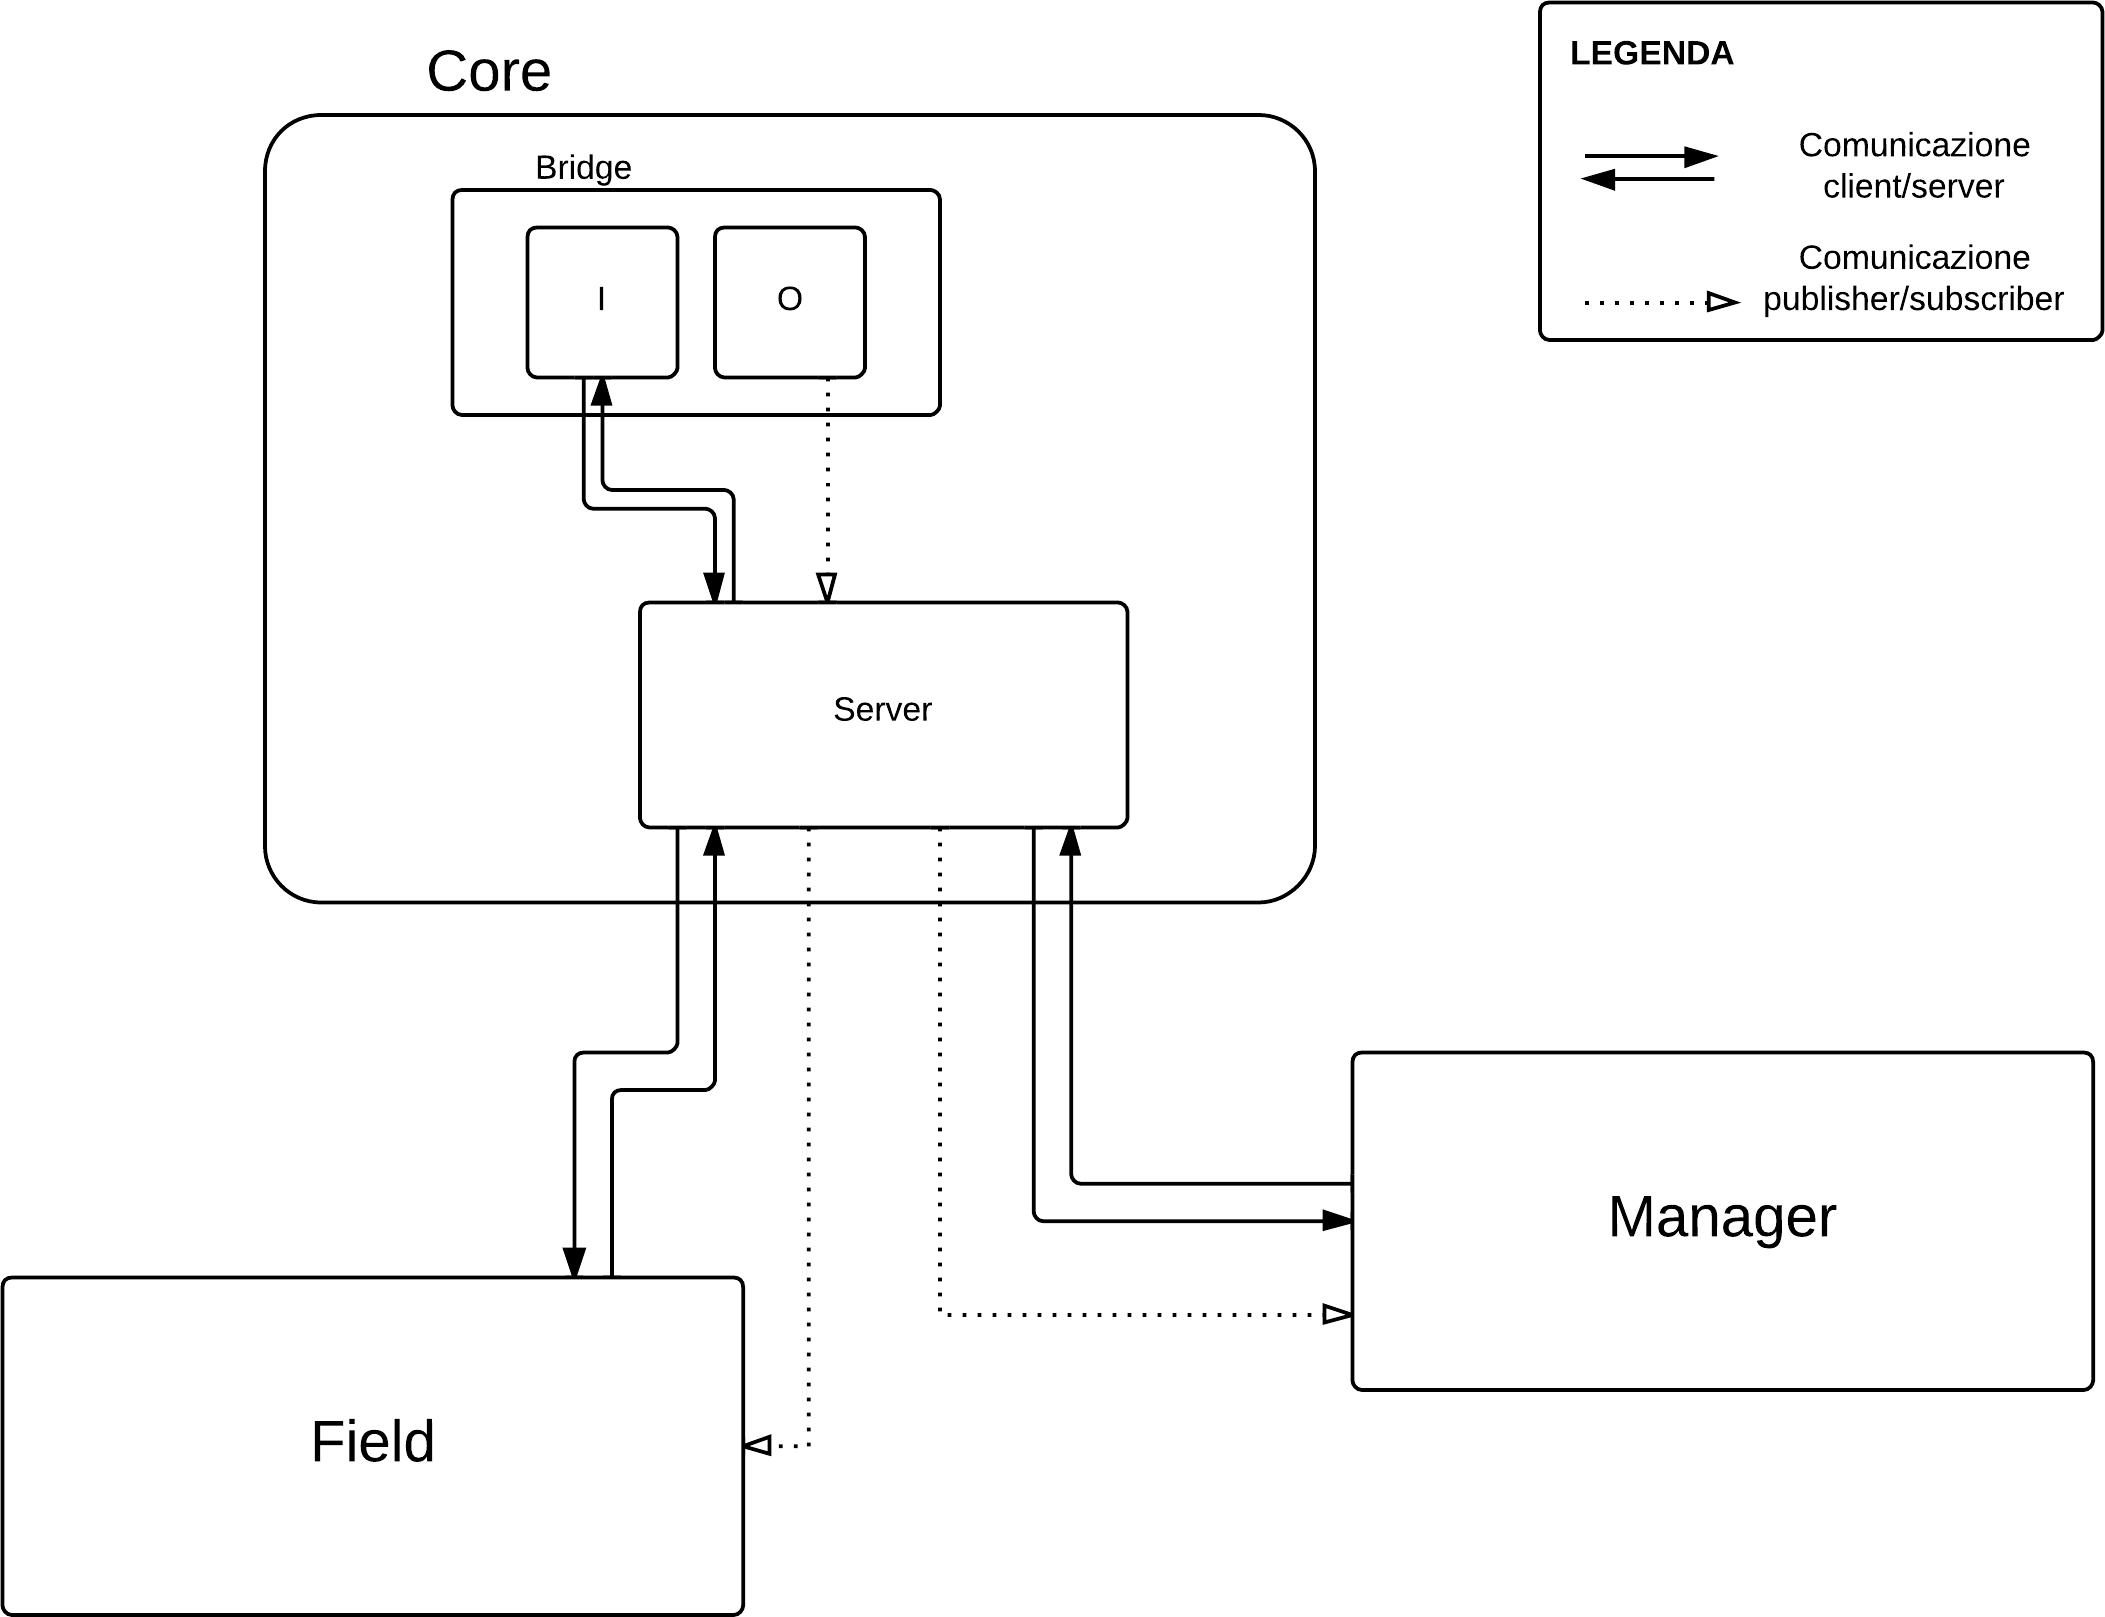
\includegraphics[scale=.21]{images/distribution_model}
	\caption{Diagramma della comunicazione tra le componenti distribuite.}
	\label{fig:distribuzione_analisi_workflow}
\end{figure}
